\documentclass[xcolor=pdftex,dvipsnames,table,final]{beamer}
\mode<presentation>
{
  \usetheme{PosterCERG}
}
% size in width and height is in cm
% Arch D: 24"x36" use 60.96 x 91.44 Typical size for our printer, use 3 columns, scale=0.8 to fit more text
% each column should be 0.3\linewidth
% Arch E: 36"x48" use 91.44 x 121.92 OK for FedexKinko, use 4 columns
% each column should be 0.22\linewidth
\usepackage[orientation=portrait,size=custom,width=76.2,height=106.68,scale=1]{beamerposter}
% DATE-2016 Poster format
% DIN-A0-Portrait ----1189mm X 841mm or 118.9cm x 84.1cm or 46.8in x 33.1in 
%\usepackage[orientation=portrait, size=custom, width=84.1, height=118.9 scale=1.0]{beamerposter}sd
\usepackage{multirow,wrapfig}
\usepackage[labelformat=empty,justification=centering]{caption}
\usepackage{tikz}
\usepackage{lmodern}
\usepackage{multirow}
\usepackage{listings}
\usetikzlibrary{fit,arrows,calc,positioning}
%\usepackage{wrapfig}
%%%%%%%%%%% Additional packages-Panci
\usepackage[T1]{fontenc}

\definecolor{ocean}{RGB}{0,205,255}
\definecolor{beamerbackground}{rgb}{0.5,0.5,0.3}
\newcommand{\rb}[1]{\raisebox{1.3ex}[-1.3ex]{#1}}

\newcommand{\urlwofont}[1] { \urlstyle{same}\url{#1} }
     
\graphicspath{{figures/}}
\title{\LARGE Flexible, Opensource workBench fOr Side-channel analysis\\ \vspace{0.5ex}(FOBOS)}
\author{Rajesh Velegalati, Panasayya Yalla, Jens-Peter Kaps}%\vspace{-2ex}
\institute{\vspace{-1ex}Department of Electrical and Computer Engineering, George Mason University, Fairfax, Virginia 22030, USA
           %\{pyalla, ehomsiri, jkaps\}@gmu.edu \url{http://cryptography.gmu.edu}
          } %this should be GMU etc. 
\date{March}

\begin{document}
\lstset{%
  basicstyle=\ttfamily,
  language=bash,
  commentstyle=\color{tabutter},
  keywordstyle=\color{black},
  numberstyle=\color{cergbg1},
  stringstyle=\color{ta3orange},
  identifierstyle=\color{cergbg1}
}
\begin{frame}[fragile]{} 
  \begin{columns}[t]
% ---------------------------------------------------------------------------
%   FIRST COLUMN
% ---------------------------------------------------------------------------
    \begin{column}{.31\linewidth}

% ---------------------------------------------------------------------------
      \begin{block}{Abstract}
Side-channel analysis (SCA) attacks pose a growing threat to the
implementations of cryptographic algorithms in software as well as in
hardware. Current standard side-channel evaluation boards with Field
Programmable Gate Arrays (FPGAs), that allow for exploring the
vulnerability of cryptographic implementations on FPGAs, are expensive
and available only for a few FPGA devices. Furthermore, a complete
open source software package that includes drivers that run test cases
on the board, control the measurement equipment, and contain several
SCA techniques, are not readily available. Each user has to assemble
his/her own setup based on software packages from multiple sources,
written in multiple languages and/or write parts of the code
themselves. Additionally, this complexity and cost makes it very
difficult, if not impossible, to educate students on SCA through
hands-on laboratory exercises. 
FOBOS is an open-source framework for
conducting SCA attacks on FPGAs which supports multiple FPGA devices
and includes all necessary software to run Differential Power Analysis
(DPA) attacks, which are the most prominent kind of SCA attacks.
Through its completeness and support for educational FPGA boards it is
an ideal teaching tool.


      \end{block}
	 
%---------------------------------------------------------------------------------

      \begin{block}{Side Channel Analysis (SCA)}
          %\vspace{-1ex}
        \begin{itemize}
          \item {\color{red}Danger:} Implementations are susceptible to Side Channel Analysis (SCA).
        \end{itemize}

        \vspace{-2ex}
        \begin{minipage}[t]{0.62\linewidth}
          %\vspace{-5cm}%\small
          \begin{itemize}
            \item Key~space~256-bit,~$2^{256} = 1.2 \cdot 10^{77}$keys
            \item Atoms in Universe {\tiny(wikipedia)} $9.4 \cdot 10^{79}$
            \item SCA allows to attack 8-bit at a time
            \item SCA complexity $\frac{256}{8} \cdot 2^{8} = 8192$
          \end{itemize}
        \end{minipage}%
        %\hspace{-0.5cm}
        \begin{minipage}[t]{0.38\linewidth}  
          \vspace{-1ex}%
          \hspace{-1ex}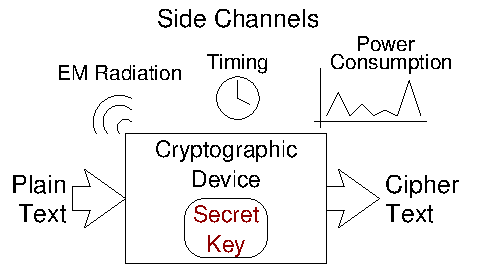
\includegraphics[width=\linewidth]{../figures/sidechannel2}
        \end{minipage}
        
        \begin{center}
        \begin{minipage}[t]{0.9\linewidth}  
        \setbeamercolor{padding}{fg=white, bg=cergbg1}
        \begin{beamercolorbox}[rounded=true]{padding}
          %\begin{block}{Danger}
          %\small%
          \begin{itemize}
            \item These are passive, non invasive attacks.
            \item They are difficult to detect.
            \item The measurement setup is not very expensive.
            \item Applies to Software as well as Hardware implementations.
          \end{itemize}
          %\end{block}
        \end{beamercolorbox}
        \end{minipage}
        \end{center}
      \end{block}
%-----------------------------------------------------------------------------------
      \begin{block}{Current SCA Evaluation Solutions}
        {\large\textbf{Hardware (FPGAs)}}%\vspace{1ex}
        \begin{itemize}
          \item Homegrown platforms or 
          \item SAKURA Boards (starting at \$1,500, or donation)
        \end{itemize}
        \begin{center}
        { \small%
          \renewcommand\tabcolsep{4pt}% 
          \rowcolors{3}{RoyalBlue!5}{RoyalBlue!20}%
          \begin{tabular}{|r||c|c|c|c||c|c}\hline
            \rowcolor{RoyalBlue!20}%
              & \multicolumn{4}{>{\columncolor{RoyalBlue!20}}c||}{\textbf{SASEBO}} 
              & \multicolumn{2}{>{\columncolor{RoyalBlue!20}}c}{\textbf{SAKURA}}      \\ 
            \rowcolor{RoyalBlue!20}%
            \rb{\textbf{Board}}   &          & \textbf{G} & \textbf{GII}  & \textbf{B}   & \textbf{X}   & \textbf{G}    \\ \hline
            \textbf{Control}      & Virtex-2 & Virtex-2   &               &              &              &               \\
            \rowcolor{RoyalBlue!5}%
            \textbf{FPGA}         & Pro      & Pro        &\rb{Spartan-3A}&\rb{Stratix-2}&\rb{Spartan-6}&\rb{Spartan-6} \\
            \rowcolor{RoyalBlue!20}%
            \textbf{DUT}          & Virtex-2 & Virtex-2   &               &              &              &               \\
            \textbf{FPGA}         & Pro      & Pro        &\rb{Virtex-5}  &\rb{Stratix-2}&\rb{Kintex-7} &\rb{Spartan-6} \\ 
            \textbf{Techn.}       
              & \multicolumn{1}{>{\columncolor{RoyalBlue!5}}r|}{130\,nm}  
              & \multicolumn{1}{>{\columncolor{RoyalBlue!5}}r|}{130\,nm}  
              & \multicolumn{1}{>{\columncolor{RoyalBlue!5}}r|}{65\,nm}        
              & \multicolumn{1}{>{\columncolor{RoyalBlue!5}}r||}{90\,nm}       
              & \multicolumn{1}{>{\columncolor{RoyalBlue!5}}r|}{28\,nm}    
              & \multicolumn{1}{>{\columncolor{RoyalBlue!5}}r}{45\,nm} \\       
                                  &          & RS232,     &               & RS232,       &              &               \\
            \rowcolor{RoyalBlue!20}%
            \rb{\textbf{PC Data}} &RS232     &FT245RL     &\rb{FT2232D}   & FT245RL      & USB          & USB           \\ 
            \rb{\textbf{Comms.}}  &          &(USB)       &\rb{(USB)}     & (USB)        &              &               \\ 
                                  &Discon-   &Discon-     &Discon-        &              &              &               \\ 
            \rowcolor{RoyalBlue!5}%
            \rb{\textbf{Status}}  &tinued    &tinued      &tinued         &              &              &               \\ \hline
          \end{tabular}
        }
        \end{center}
        {\large\textbf{Software}}%\vspace{1ex}
        \begin{itemize}
            \item The DUT is driven and power data acquired by
            \begin{itemize}
                \item Homegrown data acquisition software,
                \item Modified SASEBO software written in C\#, or
            \end{itemize}
        \end{itemize}
        \begin{center}
        \begin{minipage}[t]{0.9\linewidth}  
        \setbeamercolor{padding}{fg=white, bg=cergbg1}
        \begin{beamercolorbox}[rounded=true]{padding}
          \textbf{IA Meter}
          {\small
          \begin{itemize}
            \item Opensource set of Python scripts for acquisition and storage.
            \item Mostly independent of hardware platform and oscilloscope.
          \end{itemize}
          }
        \end{beamercolorbox}
        \end{minipage}
        \end{center}

        \begin{itemize}
            \item The data is analyzed either by
            \begin{itemize}
                \item Homegrown analysis software or
            \end{itemize}
        \end{itemize}
        \begin{center}
        \begin{minipage}[t]{0.9\linewidth}  
        \setbeamercolor{padding}{fg=white, bg=cergbg1}
        \begin{beamercolorbox}[rounded=true]{padding}
          \textbf{OpenSCA Toolbox}
          {\small
          \begin{itemize}
            \item Opensouce Matlab codes to perform DPA attacks.
            \item Supports first, higher order, and template attacks.
          \end{itemize}
        }
        \end{beamercolorbox}
        \end{minipage}
        \end{center}
        {\large\textbf{Commercial Solutions}}%\vspace{1ex}
        \begin{itemize}
          \item Cryptography Research: DPA Workstation\texttrademark
          \item Riscure: Inspector
          \item Secure IC: Smart SIC Analyzer 
        \end{itemize}
      \end{block}
%------------------------------------------------------------------------------------
          \begin{block}{Drawbacks of Current Solutions}   
          %\vspace{-1ex}
            \begin{itemize}
              \item Commercial Solutions are too expensive for educational use and for
                    many research groups

              \item IA Meter only performs acquisition using Python.
              \item OpenSCA Toolbox performs only analysis using Matlab.
              \item SAKURA has very limited FPGA support and uses C\#.
              \begin{itemize}
                \item DPA resistance depends on FPGA family.
                \item DPA resistance depends on FPGA packaging (e.g., w/ or w/o capacitances).
              \end{itemize}
              \item Currently only a patchwork of scripts and tools exist.
              \item No complete, free, and open-source solution is available.
              \item No inexpensive out-of-the-box solution for education.
            \end{itemize}
	    \vspace{0.8ex}
          \end{block}
        
%---------------------------------------------------------------------------------
    \end{column}
% ---------------------------------------------------------------------------
%   SECOND COLUMN
% ---------------------------------------------------------------------------
    \begin{column}{.31\linewidth}
   
% ---------------------------------------------------------------------------
      
% ---------------------------------------------------------------------------
      \begin{block}{FOBOS}
        {\color{red}F}lexible {\color{red}O}pen-source work{\color{red}B}ench 
        f{\color{red}O}r {\color{red}S}ide-channel analysis, 
          loosely named after the Greek god Phobos ($\phi \acute{o} \beta o \varsigma$) is 
          an open-source framework for DPA with the following goals: 
        \begin{itemize}
          \item Complete solution useful for education.
          \item De-couples Control from Device under Test (DUT).
          \item Allows use of inexpensive FPGA boards.
          \item Modular software, allows for easy adaptation for new boards, oscilloscopes.
          \item Extensible by the user to include
          \begin{itemize}
            \item new attack scenarios and
            \item new attack models. 
          \end{itemize}
        \end{itemize}
      \end{block}
% ---------------------------------------------------------------------------
      \begin{block}{Main Components of FOBOS}
        \begin{center}
          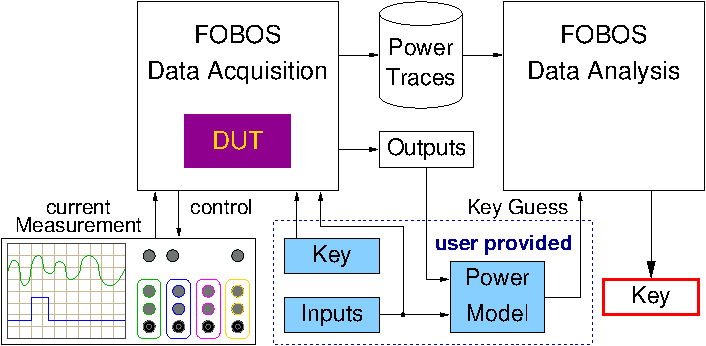
\includegraphics[scale=1.5]{../figures/fobos-top}
        \end{center} 
      \end{block}
     
% ---------------------------------------------------------------------------
      \begin{block}{FOBOS Acquisition}
        \begin{center}
          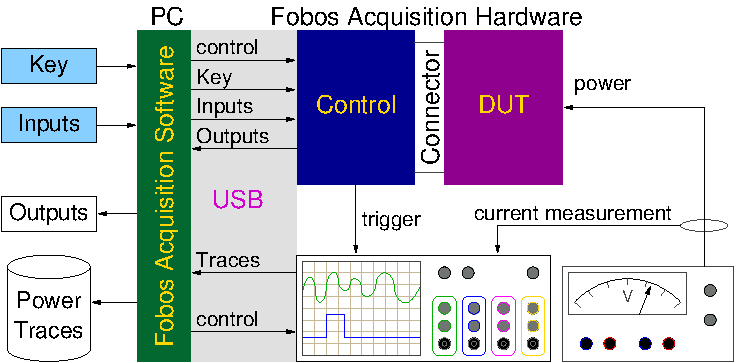
\includegraphics[scale=1.5]{../figures/fobos-dac}
        \end{center} 

          \begin{itemize}
            \item FOBOS Acquisition Hardware contains 
            \begin{itemize}
              \item VHDL for the \textbf{Control Board} to interface with DUT,
              \item VHDL-wrapper for the \textbf{DUT board} to instantiate a user provided algorithm, and
              \item Connector description.
            \end{itemize}
            \item FOBOS Acquisition Software is written in Python and 
            \begin{itemize}
              \item Controls FOBOS Acquisition Hardware,
              \item Controls measurement equipment, and
              \item Stores measurements and setup information.
            \end{itemize}
          \end{itemize}
       \end{block}
     
% ---------------------------------------------------------------------------
      \begin{block}{FOBOS Hardware}
        \vspace{-1ex}
        \begin{center}
          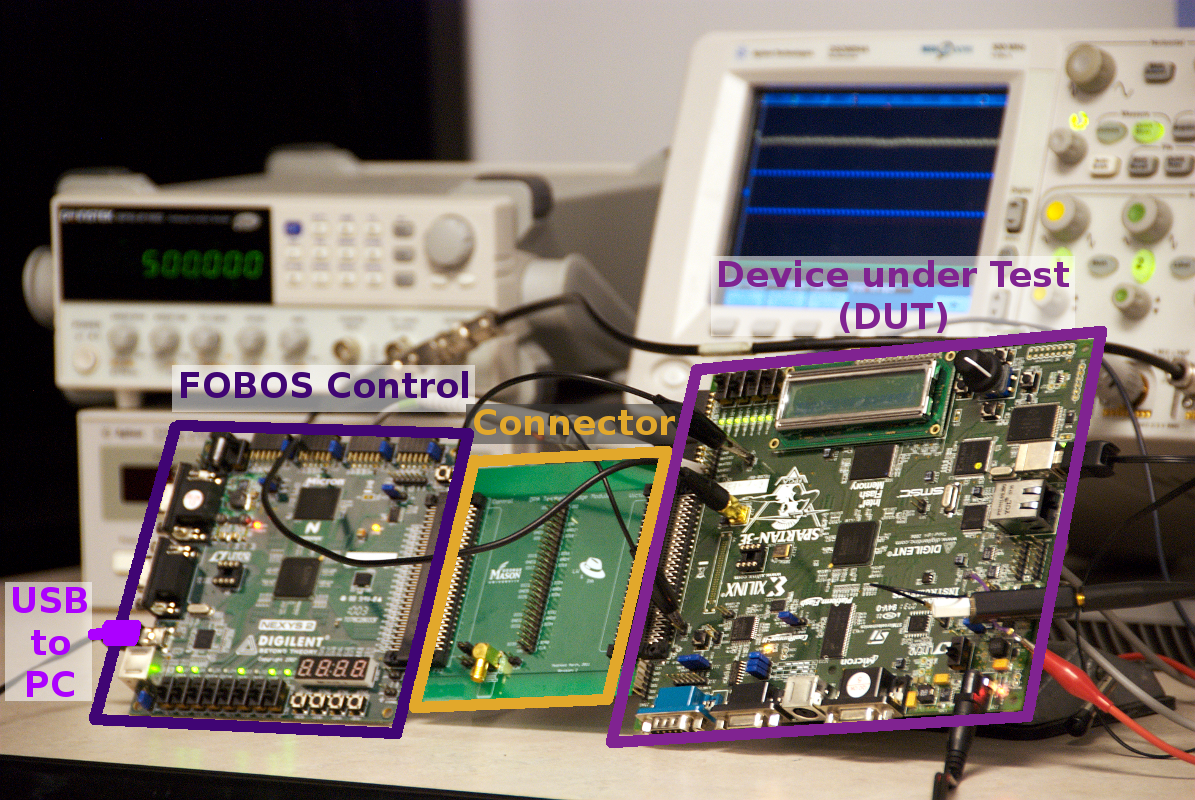
\includegraphics[width=0.9\linewidth]{../figures/FOBOS-label}
        \end{center} 
        \begin{itemize}
          \item FOBOS Control can be Digilent Nexys2 or Nexys3, soon Nexys4.
        \end{itemize}
        \vspace{-0.2ex}
       \end{block}
     
% ---------------------------------------------------------------------------
      \begin{block}{Acquisition Control}
        \begin{center}
          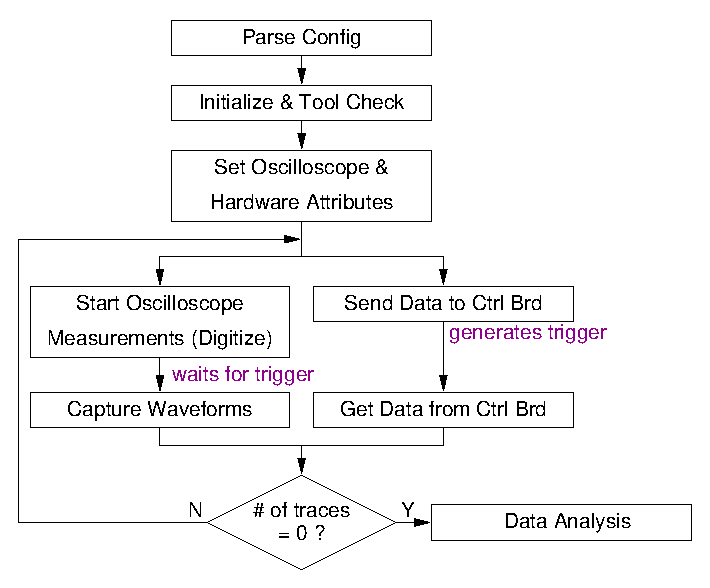
\includegraphics[scale=1.5]{../figures/data_acq}
        \end{center} 
        \begin{itemize}
          \item Control Board sends Key and Plaintext to the DUT.
          \item After DUT receives all data, the Control Board generates the trigger.
          \item The trigger indicates that the cryptographic algorithm has started
                and initiates capture of data by the oscilloscope.
        \end{itemize}
       \end{block}
     
% ---------------------------------------------------------------------------
          
% ---------------------------------------------------------------------------
    \end{column}
% ---------------------------------------------------------------------------
%   THIRD COLUMN
% ---------------------------------------------------------------------------
   \begin{column}{.31\linewidth}
    
% ---------------------------------------------------------------------------
       \begin{block}{FOBOS Analysis}
        \begin{minipage}{0.69\linewidth}
		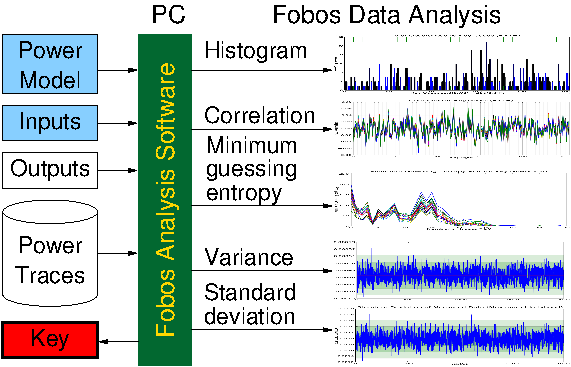
\includegraphics[scale=1.5]{../figures/fobos-dan}
        \end{minipage}
	\hspace{-5ex}
	\begin{minipage}{0.31\linewidth}
          {\small
          \begin{itemize}
            \item Minimum Guessing Entropy shows how many guesses (possible keys) are 
                  remaining for a given number of traces. 
            \item Autocorrelation indicates repeating patterns in a trace such as round 
                  operations which help in identifying where to attack. 
          \end{itemize}
          }  
	\end{minipage} 
       \end{block}
% ---------------------------------------------------------------------------
       \begin{block}{Analysis Workflow}
        \vspace{-1ex}
        \begin{center}
          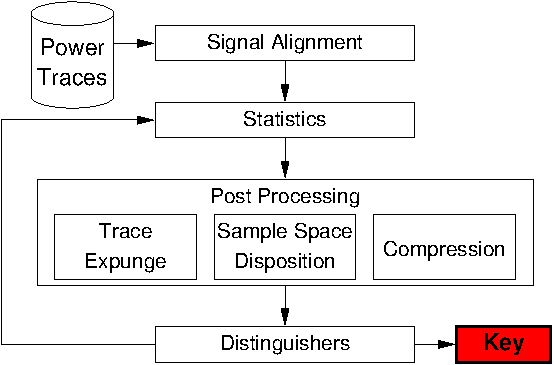
\includegraphics[scale=1.5]{../figures/data_anl}
        \end{center} 
        \vspace{-1ex}
        \begin{enumerate}
          \item Statistics Module
          \begin{itemize}
            \item Statistics can identify outliers in traces and samples across traces.
          \end{itemize}
          \item Post-Processing Module
          \begin{itemize}
            \item The main goal of these modules is to reduce the amount of data that 
                  has to be analyzed by the SCA Module.
          \end{itemize}
          \item SCA Module
          \begin{itemize}
            \item User can test his/her own power model using a library of state-of-the art side channel
                  distinguishers.
            \item FOBOS supports CPA using Spearman, Pearson, ANOVA \& MIA.
          \end{itemize}
        \end{enumerate}

       \end{block}
% ---------------------------------------------------------------------------
       \begin{block}{Signal Alignment}
        \begin{minipage}[t]{0.49\linewidth}
          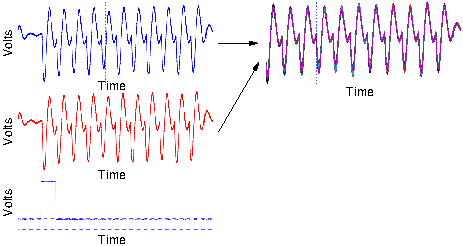
\includegraphics[scale=2.4]{../figures/tracealingment}
        \end{minipage}%
        \begin{minipage}[t]{0.49\linewidth}
         \vspace{-4cm}
         \begin{itemize}
          \item The recorded trigger signal is used by FOBOS Analysis to align the
                power traces.
         \end{itemize} 
        \end{minipage}
       \end{block}
% ---------------------------------------------------------------------------
       \begin{block}{Sample Space Disposition}
        \begin{minipage}[t]{0.49\linewidth}%
		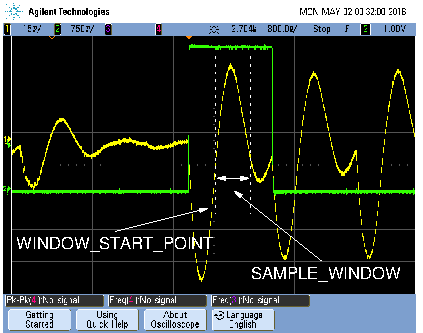
\includegraphics[width=0.9\linewidth]{../figures/oscilloscope-sample-window}
        \end{minipage}%
        \begin{minipage}[t]{0.49\linewidth}%
          \vspace{-6.5cm}% 
          \begin{itemize}
            \item User can select any part of the trace for further analysis.
            \item Reduces computation time.
          \end{itemize} 
          \begin{center}
            \setbeamercolor{padding}{fg=white, bg=cergbg3}
            \begin{beamercolorbox}[rounded=true]{padding}%
               \footnotesize%
              \begin{lstlisting}
WINDOW_START_POINT = 100
SAMPLE_WINDOW = 1000
              \end{lstlisting}
            \end{beamercolorbox}
          \end{center}
        \end{minipage}
       \end{block}
% ---------------------------------------------------------------------------
       \begin{block}{Compression}
        \begin{minipage}[t]{0.49\linewidth}
		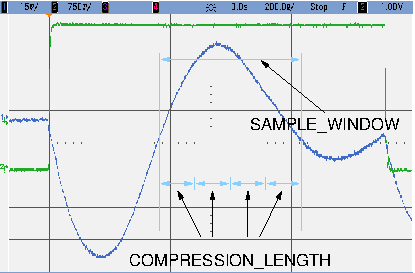
\includegraphics[width=0.9\linewidth]{../figures/oscilloscope-compression-window}
        \end{minipage}%
        \begin{minipage}[t]{0.49\linewidth}%
          \vspace{-6.5cm}% 
         \begin{itemize}
           \item Compresses length to MAXimum, MINimum, or MEAN.
%           \item Further reduces number of points for correlation.
         \end{itemize} 
          \begin{center}
            \setbeamercolor{padding}{fg=white, bg=cergbg3}
            \begin{beamercolorbox}[rounded=true]{padding}%
               \footnotesize%
              \begin{lstlisting}
COMPRESSION_LENGTH = 40
COMPRESSION_TYPE = MAX
              \end{lstlisting}
            \end{beamercolorbox}
          \end{center}
        \end{minipage}
       \end{block}
% ---------------------------------------------------------------------------
       \begin{block}{Example: Attack on AES}
        \vspace{-1ex}
         \begin{center}
           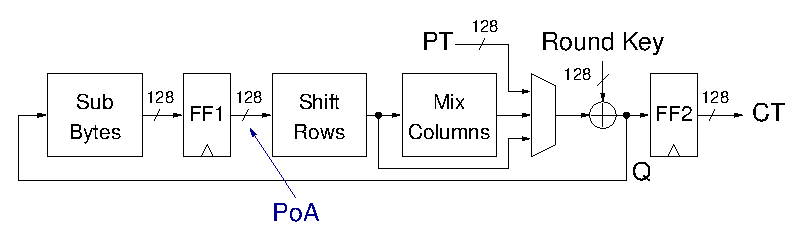
\includegraphics[width=0.9\linewidth]{../figures/aes128}

           {\small $PowerGuess_{i, j}$ = HD(SBOX($CT_{i-1}$), SBOX($PT_{i}$ $\oplus$ $KeyGuess_{j}$) )}
         \end{center}
	 \begin{minipage}[t]{0.49\linewidth}
		 %\begin{center}
			~~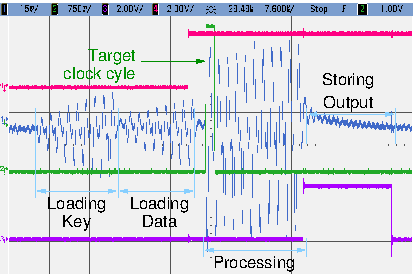
\includegraphics[width=0.80\linewidth]{../figures/oscilloscope-all-4ch} 
		%\end{center}
	 
	 \end{minipage}%
	 \begin{minipage}[t]{0.49\linewidth}  
		 \hspace{-5ex}\vspace{-6cm}{\small
		 \begin{itemize}
		  \item First round attack on AES-128.
		  \item Key (0x16) recovered after 1 hour.
                  \item Requires 2000 encryptions.
                  \item Pearson's Correlation.
                  \item Sometimes histogram is more clear than correlation plot.
		 \end{itemize}}
         \end{minipage} 
	 
        \begin{minipage}[t]{0.49\linewidth}
           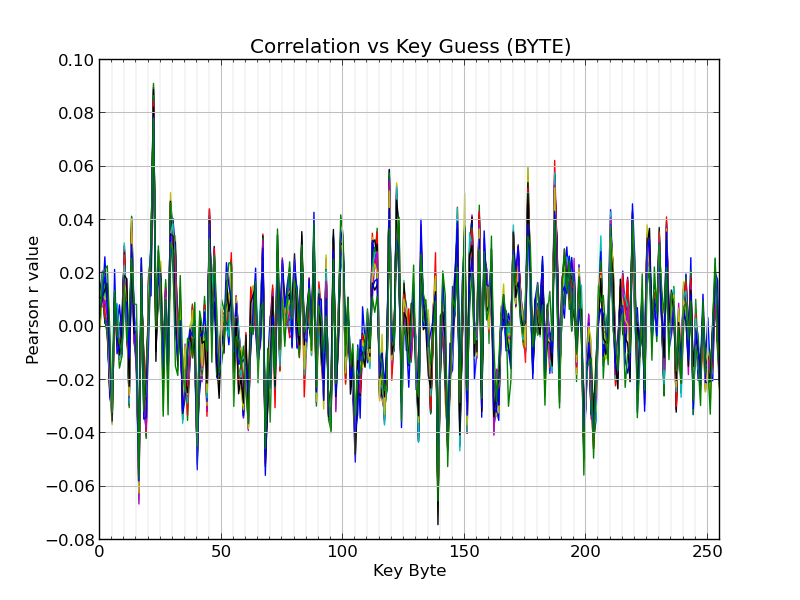
\includegraphics[width=1.0\linewidth]{../figures/pearsonsCoActual}
        \end{minipage}%
        \begin{minipage}[t]{0.49\linewidth}  
		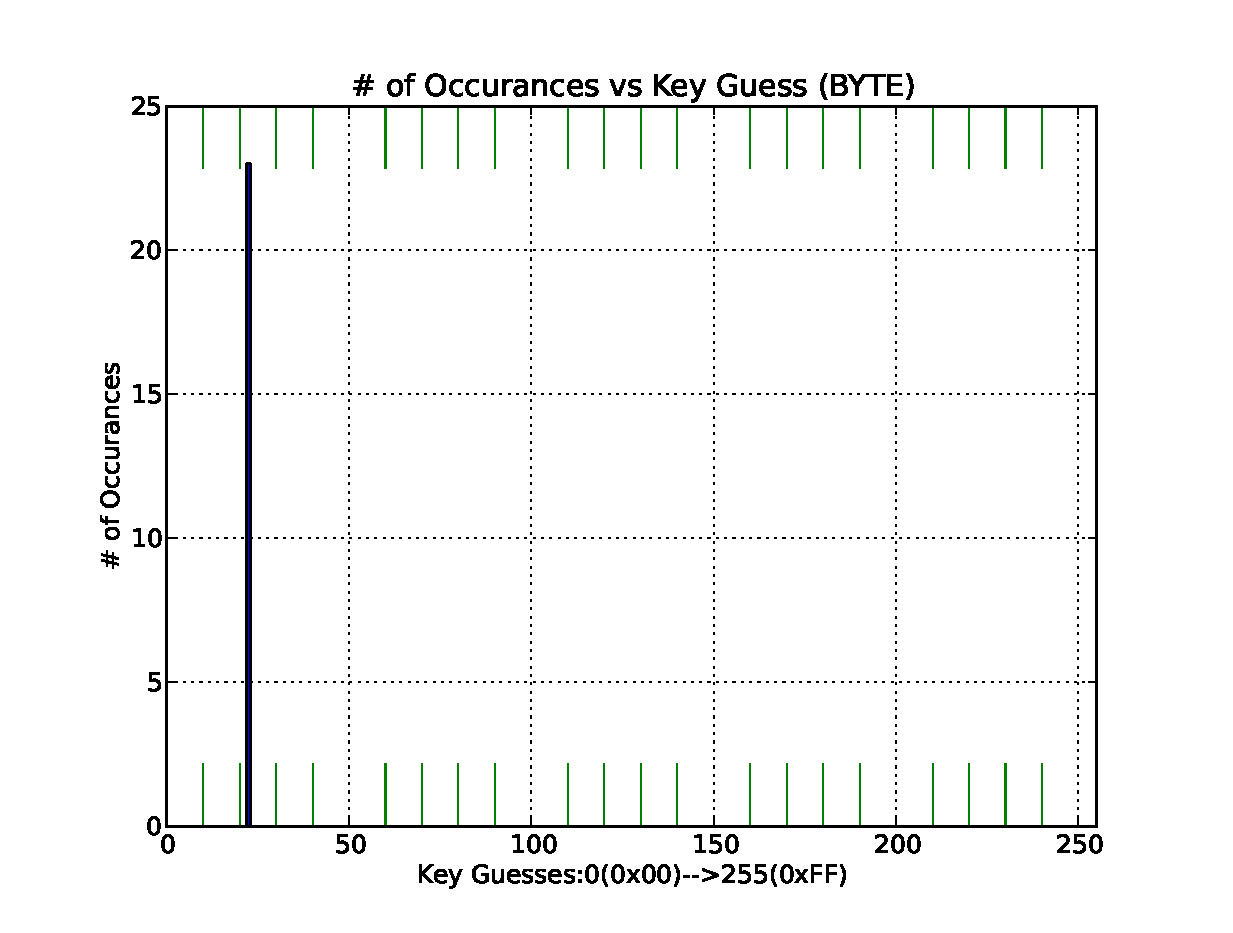
\includegraphics[width=1.0\linewidth]{../figures/histPearsonsCoActual}
        \end{minipage}
        \vspace{-3.8ex}
       \end{block}
% ---------------------------------------------------------------------------
% ---------------------------------------------------------------------------
%      \begin{block}{References}
%        \footnotesize
%          \bibliographystyle{IEEEtran}
%          \bibliography{keccak}
%        %\input{keccakbib}
%      \end{block} 
   \end{column}
\end{columns}

\end{frame}
\end{document}

 
